\documentclass[%
	11pt,
	a4paper,
	utf8,
	%twocolumn
		]{article}	

\usepackage{style_packages/podvoyskiy_article_extended}


\begin{document}
\title{Заметки по Анализу временных рядов и сопряженным вопросам}

\author{\itshape Подвойский А.О.}

\date{}
\maketitle

\thispagestyle{fancy}

Здесь приводятся заметки по некоторым вопросам, касающимся машинного обучения, анализа данных, программирования на языках \texttt{Python}, \texttt{R} и прочим сопряженным вопросам так или иначе, затрагивающим работу с временными рядами.


\shorttableofcontents{Краткое содержание}{1}

\tableofcontents

\section{Приемы работы с библиотекой ETNA}

\subsection{Полезные рерсурсы}

Домашняя страница проекта \url{https://github.com/tinkoff-ai/etna}.

\subsection{Установка}

Установить библиотеку можно как обычно с помощью менеджера пакетов \verb|pip|
\begin{lstlisting}[
style = ironpython,
numbers = none
]
pip install etna
\end{lstlisting}

\subsection{Сжатая сводка по библиотеке, рекомендации}

\begin{itemize}
	\item Перекрестную проверку с расширяющимся окном (или на скользящем окне) в библиотеке ETNA можно выполнить с помощью метода \verb|backtest()|. 
	
	\item Размер тестовой выборки, как правило, определяется \emph{горизонтом прогнозирования} $ h $, а тот в свою очередь определяется бизнес-требованиями. Если, скажем, интересует прогноз на 14 дней вперед, то и тестовая выборка должна включать 14 более поздних наблюдений.
	
	\item Размер тестовой выборки остается постоянным. Это значит, что метрики качества, полученные в результате вычислений прогнозов каждой обученной модели по тестовому набору, будут последовательны и их можно объединять и сравнивать.
	
	\item Размер обучающей выборки не может быть меньше тестовой выборки.
	
	\item Если данные содержат сезонность, обучающая выборка должна содержать не менее двух полных сезонных циклов (правило $ 2 L $, где $ L $ -- количество периодов в полном сезонном цикле, необходимое для инициализации параметров некоторых моделей, например, для вычисления исходного значения тренда в модели тройного экспоненциального сглаживания), учитывая уменьшение длины ряда при выполнении процедур обычного и сезонного дифференциирования.
	
	\item {\color{blue} \underline{Ширина окна} $ w $ для скользящих статистик (и лаговых признаков) должна быть неменьше горизонта прогнозирования, $ w \geqslant h $ (видимо, для того чтобы поймать паттерн соответствующего горизонта, например, недельный). И \underline{порядок лага} $ lag\_ord $ должен быть неменьше горизонта прогнозирования $ lag\_ord \geqslant h $. Так как в противном случае признаки тестового поднабора данных, построенные на лагах с порядком меньшим горизонта прогнозирования, будут использовать значения целевой переменной из тестового поднабора данных (а это утечка)}.
	
	\item Скользящее среднее используется не только для конструирования признаков, но и в качестве прогнозной модели\footnote{Как и фильтр Калмана, и преобразование Фурье} (когда прогноз -- это скользящее среднее $ n $ последних наблюдений), а также для сглаживания выбросов, краткосрочных колебаний и более четкого выделения долгосрочных тенденций в ряде.
\end{itemize}

\subsection{Примеры использования}

\subsubsection{Начало}

Кадр данных, представляющих временной ряд должен содержать следующие столбцы:
\begin{itemize}
	\item \verb|target|: столбец, который нужно предсказывать,
	
	\item \verb|timestamp|: столбец с временными метками,
	
	\item \verb|segment|: имя сегмента, так как в общем случае ETNA ориентируется на многомерные временные ряды. В случае одномерного ряда получается такой вот атрибут-артефакт.
\end{itemize}

\begin{lstlisting}[
style = ironpython,
numbers = none	
]
import pandas as pd

original_df = pd.read_csv("data/monthly-australian-wine-sales.csv")
# month -> timestamp, sales -> target
original_df["timestamp"] = pd.to_datetime(original_df["month"])
original_df["target"] = original_df["sales"]
original_df.drop(columns=["month", "sales"], inplace=True)
original_df["segment"] = "main"
\end{lstlisting}

Библиотека ETNA работает со специальной структурой данных \verb|TSDataset|, поэтому сначала классический \verb|DataFrame| преобразовать в \verb|TSDataset|
\begin{lstlisting}[
style = ironpython,
numbers = none
]
from etna.datasets.tsdataset import TSDataset

original_df: pd.DataFrame
df: pd.DataFrame = TSDdataset.to_dataset(original_df)
\end{lstlisting}

А вот теперь можно построить \verb|TSDataset|
\begin{lstlisting}[
style = ironpython,
numbers = none
]
ts: TSDataset = TSDataset(df, freq="MS")
\end{lstlisting}

Можно посмотреть базовую инфомрацию
\begin{lstlisting}[
style = ironpython,
numbers = none
]
ts.info()
"""
<class 'etna.datasets.TSDataset'>
num_segments: 1
num_exogs: 0
num_regressors: 0
num_known_future: 0
freq: MS
start_timestamp end_timestamp  length  num_missing
segments                                                   
main          1980-01-01    1994-08-01     176            0
"""
\end{lstlisting}

Или в формате кадра данных
\begin{lstlisting}[
style = ironpython,
numbers = none
]
ts.describe()
\end{lstlisting}

Построим прогноз с помощью простой модели \verb|NaivModel|
\begin{lstlisting}[
style = ironpython,
numbers = none
]
train_ts, test_ts = ts.train_test_split(
    train_start="1980-01-01",
    train_end="1993-12-01",
    test_start="1994-01-01",
    test_end="1994-08-01",
)
\end{lstlisting}

\begin{lstlisting}[
style = ironpython,
numbers = none	
]
from etna.models import NaiveModel
HORIZON = 8

# Fit the model
model = NaiveModel(lag=12)
model.fit(train_ts)

# Make the forecast
future_ts = train_ts.make_future(
    future_steps=HORIZON,
    tail_steps=model.context_size
)
forecast_ts = model.forecast(
    future_ts,
    prediction_size=HORIZON
)
\end{lstlisting}

Оценим качество прогноза
\begin{lstlisting}[
style = ironpython,
numbers = none
]
from etna.metrics import SMAPE

smape = SMAPE()
smape(y_true=test_ts, y_pred=forecast_ts)  # {'main': 11.492045838249387}
\end{lstlisting}

Теперь построим прогноз с помощью Catboost
\begin{lstlisting}[
style = ironpython,
numbers = none
]
from etna.transforms import LagTransform, LogTransform

lags = LagTransform(
    in_column="target",
    lags=list(rante(8, 24, 1))
)
log = LogTransform(in_column="target")
transforms = [log, lags]
# Преобразования применяются к обчающему фрагменту ряда на месте
train_ts.fit_transform(transforms)
\end{lstlisting}

\begin{lstlisting}[
style = ironpython,
numbers = none
]
from etna.models import CatBoostMultiSegmentModel

model = CatBoostMultiSegmentModel()
model.fit(train_ts)
future_ts = train_ts.make_future(future_steps=HORIZON, transforms=transforms)
forecast_ts = model.forecast(future_ts)
forecast_ts.inverse_transform(transforms)
\end{lstlisting}

\begin{lstlisting}[
style = ironpython,
numbers = none
]
from etna.metrics import SMAPE

smape = SMAPE()
smape(y_true=test_ts, y_pred=forecast_ts)  # {'main': 10.657026308972483}
\end{lstlisting}

Все шаги можно собрать в конвейер
\begin{lstlisting}[
style = ironpython,
numbers = none	
]
from etna.pipeline import Pipeline

train_ts, test_ts = ts.train_test_split(
	train_start="2019-01-01",
	train_end="2019-10-31",
	test_start="2019-11-01",
	test_end="2019-11-30",
)

model = Pipeline(
	model=CatBoostMultiSegmentModel(),
	transforms=transforms,
	horizon=HORIZON,
)
model.fit(train_ts)
forecast_ts = model.forecast()

smape = SMAPE()
smape(y_true=test_ts, y_pred=forecast_ts)
\end{lstlisting}

\subsection{Обратное тестирование. Backtest}

\begin{lstlisting}[
style = ironpython,
numbers = none
]
import pandas as pd
import matplotlib.pyplot as plt

from etna.datasets.tsdataset import TSDataset
from etna.metrics import MAE
from etna.metrics import MSE
from etna.metrics import SMAPE
from etna.pipeline import Pipeline
from etna.models import ProphetModel
from etna.analysis import plot_backtest
\end{lstlisting}

Пример обратного тестирования на 3-х фолдах (\pic{fig:backtest}).

\begin{figure}[h]
	\centering
	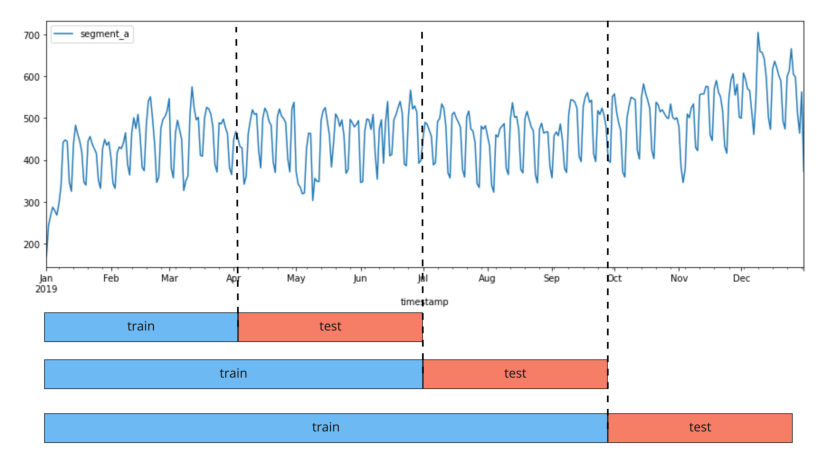
\includegraphics[scale=1.0]{figures/backtest.png}
	\caption{ Обратное тестирование на 3-х фолдах }\label{fig:backtest}
\end{figure}

\begin{lstlisting}[
style = ironpython,
numbers = none
]
df = pd.read_csv("./data/example_dataset.csv")
df = TSDataset.to_dataset(df)
ts = TSDataset(df, freq="D")
\end{lstlisting}

Создадим цепочку преобразований
\begin{lstlisting}[
style = ironpython,
numbers = none
]
horizon = 31  # Set the horizon for predictions
model = ProphetModel()  # Create a model
transforms = []  # A list of transforms -  we will not use any of them

pipeline = Pipeline(model=model, transforms=transforms, horizon=horizon)
\end{lstlisting}

Метод \verb|backtest()| возвращает три кадра данных:
\begin{itemize}
	\item кадр данных с метриками для каждого фолда и каждого сегмента,
	
	\item кадр данных с прогнозами,
	
	\item кадр данных с информацией по каждому фолду.
\end{itemize}

\begin{lstlisting}[
style = ironpython,
numbers = none
]
metrics_df, forecast_df, fold_info_df = pipeline.backtest(
    ts=ts,
    metrics=[
        MAE(),
        MSE(),
        SMAPE(),
    ]
)
\end{lstlisting}

Можно получить метрики, усредненные по фолдам
\begin{lstlisting}[
style = ironpython,
numbers = none
]
metrics_df, forecast_df, fold_info_df = pipeline.backtest(
    ts=ts,
    metrics=[
        MAE(),
        MSE(),
        SMAPE()
    ],
    aggregate_metrics=True,
)
\end{lstlisting}

Обратное тестирование с масками для фолдов. Рассмотрим 3 стратегии: \verb|SlidingWindowSplitter|, \verb|ExpandingWindowSplitter| и \verb|SingleWindowSplitter| (из \verb|sktime|).

Чтобы использовать стратегию расширяющегося окна \verb|ExpandingWindowSplitter|, достаточно просто использовать \verb|mode="expand"|
\begin{lstlisting}[
style = ironpython,
numbers = none
]
metrics_df, _, _ = pipeline.backtest(
    ts=ts,
    metrics=[
        MAE(),
        MSE(),
        SMAPE()
    ],
    n_folds=3,
    mode="expand"
)
\end{lstlisting}

Для того чтобы использовать стратегию \verb|SlidingWindowSplitter|
\begin{lstlisting}[
style = ironpython,
numbers = none
]
from etna.pipeline import FoldMask
import numpy as np

# 1 Without mask
metrics_df, _, _ = pipeline.backtest(
    ts=ts,
    metrics=[
        MAE(),
        MSE(),
        SMAPE()
    ],
    n_folds=1
)
\end{lstlisting}

Или с маской
\begin{lstlisting}[
style = ironpython,
numbers = none
]
# 2 With specific mask
window_size = 85
first_train_timestamp = ts.index.min() + np.timedelta64(100, "D")
last_train_timestamp = first_train_timestamp + np.timedelta64(window_size, "D")
target_timestamps = pd.date_range(start=last_train_timestamp + np.timedelta64(1, "D"), periods=horizon)
mask = FoldMask(
	first_train_timestamp=first_train_timestamp,
	last_train_timestamp=last_train_timestamp,
	target_timestamps=target_timestamps,
)

metrics_df, _, _ = pipeline.backtest(ts=ts, metrics=[MAE(), MSE(), SMAPE()], n_folds=[mask])
\end{lstlisting}

Чтобы использовать стратегию скользящего окна \verb|SlidingWindowSplitter|, нужно создать список масок для фолдов \verb|FoldMask|
\begin{lstlisting}[
style = ironpython,
numbers = none
]
n_folds = 3

def sliding_window_masks(window_size, n_folds):
	masks = []
	for n in range(n_folds):
		first_train_timestamp = ts.index.min() + np.timedelta64(100, "D") + np.timedelta64(n, "D")
		last_train_timestamp = first_train_timestamp + np.timedelta64(window_size, "D")
		target_timestamps = pd.date_range(start=last_train_timestamp + np.timedelta64(1, "D"), periods=horizon)
		mask = FoldMask(
			first_train_timestamp=first_train_timestamp,
			last_train_timestamp=last_train_timestamp,
			target_timestamps=target_timestamps,
		)
		masks.append(mask)
		return masks
\end{lstlisting}

\begin{lstlisting}[
style = ironpython,
numbers = none
]
masks = sliding_window_masks(window_size=window_size, n_folds=n_folds)
metrics_df, _, _ = pipeline.backtest(ts=ts, metrics=[MAE(), MSE(), SMAPE()], n_folds=masks)
\end{lstlisting}






\listoffigures\addcontentsline{toc}{section}{Список иллюстраций}

% Источники в "Газовой промышленности" нумеруются по мере упоминания 
\begin{thebibliography}{99}\addcontentsline{toc}{section}{Список литературы}
	\bibitem{lutz:learningpython-2011}{\emph{Лутц М.} Изучаем Python, 4-е издание. -- Пер. с англ. -- СПб.: Символ-Плюс, 2011. -- 1280~с. }
	
	\bibitem{geron:hands_on_ml}{\emph{Жерон О.} Прикладное машинное обучение с помощью Scikit-Learn и TensorFlow: концепции, инструменты и техники ля создания интеллектуальных систем. -- СПб.: ООО <<Альфа-книга>>, 2018. -- 688 с.}
	
	\bibitem{burkov:2020}{\emph{Бурков А.} Машинное обучение без лишних слов. -- СПб.: Питер, 2020. -- 192 с.}
	
	\bibitem{burkov-engineer:2022}{\emph{Бурков А.} Инженерия машинного обучения. -- М.:ДМК Пресс, 2022. -- 306 с.}
	
	\bibitem{lakshmanan-mldp:2022}{\emph{Лакшманан В.} Машинное обучение. Паттерны проектирования. -- СПб.: БХВ-Перетбург, 2022. -- 448 с.}
		
	\bibitem{beazley:python-2010}{\emph{Бизли Д.} Python. Подробный справочник. -- Пер. с англ. -- СПб.: Символ-Плюс, 2010. -- 864~с. }
	
	\bibitem{dart:2015}{\emph{Rashmi K.V.}, \emph{Gilad-Bachrach R.} DART: Dropouts meet Multiple Additive Regression Trees, 2015}
	
	\bibitem{ke-lightgbm:2017}{\emph{Ke G. etc.} LightGBM: A Highly Efficient Gradient Boosting Decision Tree, 2017}
\end{thebibliography}

\end{document}
